\chapter{Topic Modelling}
\label{cha:topic_modelling}
In this chapter, we use a topic model to find themes/topics that exist in our dataset. Our input
dataset is a set of relevant tweets as determined by the classifier in the previous chapter. We use
Latent Dirichlet Allocation as our topic model as described in \Sectionref{sec:bg_lda} on page
\pageref{sec:bg_lda}.

Tables~\ref{tab:30-topics} and~\ref{tab:40-topics} on pages \pageref{tab:30-topics} and
\pageref{tab:40-topics} each show a list of 30 and 40 topics. It also contains their respective
topic-tokens distribution. For the purpose of this study, a token is either a unigram or bigram.
Each row comprises of a list of tokens that try to explain a topic and they are ordered by their
level of influence. While it is helpful to have our tokens ordered by level of influence, the
respective influence values are excluded from the table because we will not pay much
attention to them during our analysis.

% TODO: Briefly explain methodology of analysis

\section{Preprocessing}
\label{sec:lda_preprocessing}
% TODO: Complete this section

\section{Evaluating Topic Models}
\label{sec:evaluating_topic_models}
In this section, we analyse two separate models one of which will comprise of 30 topics while the
other of 40 topics. They both use a mixture of unigrams and bigrams in their token distribution.
This was inspired by our experiments in \Sectionref{sec:training_classifier} where the classifier
showed better performance when using a mixture of unigrams and bigrams. We analyse a few topics for
each model and have a look at some of the tweets that fall under those topics.
% TODO: Something about our empirical approach to the evaluation here

\subsection{Evaluating 30 Topics}
\label{sec:evaluating-30-topics}
\begin{figure}
\begin{center}
  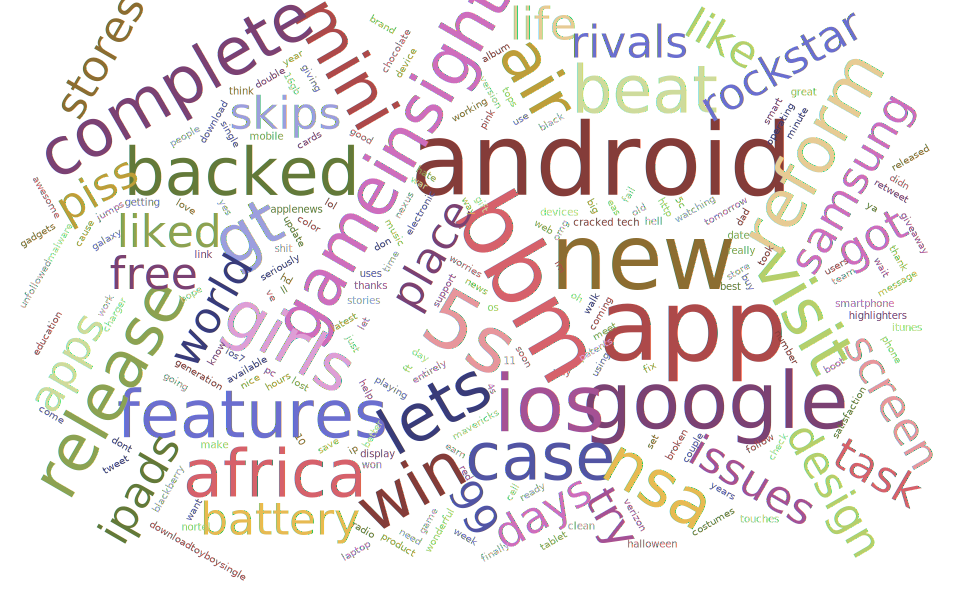
\includegraphics[scale=0.75,angle=90]{Figures/30_topics_cloud}
\end{center}
\caption{A word cloud of all tokens from all topics in our 30-topics model}
\label{fig:30-topics-cloud}
\end{figure}

The topic-word distributions in \Tableref{tab:30-topics} are a combination of unigrams
and bigrams.\\

\begin{longtable}{c p{16cm}} \toprule
  Topic & Topic-Tokens Distribution \\ \midrule
   0    & app, latest, generation, version, galaxy, won, set, oh, save, minute \\ \midrule
   1    & walk, watching, unveils, today stories, beat rivals, ipads beat, missed unveils, revamped, revamped ipads, rivals \\ \midrule
   2    & perfect, case, 16gb, black, gt, giving, clean, smartphone, ya, pink \\ \midrule
   3    & screen, place, http, better, place visit, visit gameinsight, entirely, electronic \\ \midrule
   4    & video, love, app android, yay, tomorrow, let, liked, liked video, operating, single \\ \midrule
   5    & complete, follow, managed, week, having, girls, task, complete task, managed complete \\ \midrule
   6    & ios, lets, bbm ios, ios lets, lets apps, features, game, tech, missed \\ \midrule
   7    & google, backed, google samsung, mobile, nortel, patents, microsoft backed, rockstar, backed rockstar, uses \\ \midrule
   8    & using, world, best, hate, beat, skips, skips africa, africa, africa world, release 5s \\ \midrule
   9    & music, 10, mavericks, number, yes, coming, soon, earn, cards, support \\ \midrule
   10   & new, app, store, available, design, playing, stargazing, stargazing app, new design \\ \midrule
   11   & really, os, gift, stores, hours, news, fail, stores piss, piss, broken \\ \midrule
   12   & day, battery, good, shit, display, thanks, battery life, omg, seriously, ios7 \\ \midrule
   13   & android, use, blackberry, update, web, 11, issues, devices, hd, fix issues \\ \midrule
   14   & official, 5s, 5c, life, models, cracked, color, worries, nexus, highlighters \\ \midrule
   15   & know, pc, 4s, old, does, releases, air saywhatnow, releases air, saywhatnow, did \\ \midrule
   16   & time, ll, date, wonderful, charger, working, nice, message, cell, took \\ \midrule
   17   & got, today, ve, going, smart, help, protector, hell, screen protector, got new \\ \midrule
   18   & samsung, don, download, updated, people, radio, meet, ft, updated ios, malware jumps \\ \midrule
   19   & nsa, microsoft, facebook google, google substantial, nsa surveillance, reform, reform nsa, substantial, substantial reform, surveillance \\ \midrule
   20   & lol, education, chocolate, team, double, wait, boot, white girls, girls like, couple days \\ \midrule
   21   & air, free, visit, power, satisfaction, 99 free, app 99, power tablet, tops, war \\ \midrule
   22   & release, like, new, facebook, big, make, new 5s, gadgets, product, brand \\ \midrule
   23   & just, white, app, gold, users, gold 5s, awesome, way, unfollowed, link \\ \midrule
   24   & verizon, laptop, finally, say, dont, years, getting, ready, costumes, lost \\ \midrule
   25   & apps, phone, check, ip, cause, thank, hope, dad, im, gt gt \\ \midrule
   26   & gameinsight, halloween, try, retweet, giveaway, win, work, try gameinsight, days, tweet \\ \midrule
   27   & bbm, bbm android, official release, android official, android bbm, perfect features, features bbm, want, buy, need \\ \midrule
   28   & mini, win, chance, come, chance win, case mini, kickstand, kickstand case, mini models \\ \midrule
   29   & itunes, released, think, year, great, touches, album, downloadtoyboysingle, didn, eas \\ \bottomrule
\caption{30 topic-tokens distribution with unigrams and bigrams}
\label{tab:30-topics}
\end{longtable}
%analyse 6, 7, 9, 12, 13, 14, 22, 27, 28



\subsubsection{Topic 6}
\label{sec:topic_6}
\textit{ios, lets, bbm ios, ios lets, lets apps, features, game, tech, missed} \\\\
The most common theme in the above distribution is ``ios'' and ``lets''. ``bbm'' also seems to have
a considerate amount of relevancy as it is the third most relevant token. The other tokens seem
random but we should be able to explain them better after taking a look at some of the tweets with a
fair proportion of this topic.

\begin{table}[H]
  \begin{tabular}{c c p{13cm}} \toprule
    No & Proportion & Tweet \\ \midrule
    1  & 81\%       & Fantastical 2 for iPhone gets bold iOS 7 redesign, many new features \#tech \\ \midrule
    2  & 75\%       & Limbo for iOS is now even cheaper at \$0.99 \\ \midrule
    3  & 80\%       & Don't miss out on loads of great iOS game sales from\ldots \\ \midrule
    4  & 70\%       & What new features does Apple's iOS 7 boast? \\ \midrule
    5  & 63\%       & get the BBM on iPhone iOS, lets get the apps here now \\ \midrule
    6  & 89\%       & time guessing is hard! test yourself on ur iPhone it's \#cool tweet your
    results from the app \#game \#ios \#app \\ \bottomrule
  \end{tabular}
  \caption{Tweets classified under topic 6}
  \label{tab:topic_6_tweets}
\end{table}

The tweets in \Tableref{tab:topic_6_tweets} all seem to have at least 63\% of topic 6. While they
might look like carefully selected tweets, they were actually chosen at random. Our dataset contains
a large fraction of the third, fourth and fifth tweet. Approximately 90\% of them are retweets which
explains why our topic model extracted ``ios lets'', ``lets apps'', ``game'' and ``tech'' as
relevant tokens. The sixth tweet arguably does not really have anything to do with ``iOS'' but
because it has been tagged with three words that our topic model finds salient, it gets tagged as
having 89\% proportion of topic 6.



\subsubsection{Topic 7}
\label{sec:topic_7}
\textit{google, backed, google samsung, mobile, nortel, patents, microsoft backed, rockstar, backed
rockstar, uses } \\\\
From a simple scan through the tokens in this topic, we can postulate that the tweets in this topic
will mostly be about Google, Samsung, Nortel and the Rockstar Consortium. Nortel was a
communications and networking equipment manufacturer which went bankrupt and the Rockstar Consortium
was formed to negotiate licensing for patents they owned. However, we do not expect our whole
dataset to be about patent war between these companies. Samsung and Google are large technology
companies and we might encounter tweets that simple compare their products with that of Apple. We
can make this assumption because we know our dataset is Apple-centric.

\begin{table}[H]
  \begin{tabular}{c c p{13cm}} \toprule
    No  & Proportion & Tweet \\ \midrule
    1   & 86\%       & Apple files patent for slim solar-powered technology via GigaOM \\ \midrule
    2   & 78\%       & Google, Samsung, and others sued over search patents by Apple-backed Nortel group \\ \midrule
    3   & 78\%       & Apple, Microsoft-Backed Rockstar Consortium Sues Google, Samsung Over 7 \\ \midrule
    4   & 83\%       & Apple, Microsoft-backed Rockstar uses Nortel patents to sue Google, Samsung and others \\ \midrule
    5   & 78\%       & Google Fiber comes to iPhone, iPod touch with DVR functions \\ \midrule
    6   & 80\%       & Google Replacing Android ID With Advertising ID Similar To Apple's IDFA \\ \midrule
    7   & 68\%       & Nexus 4 will get the updated ``in the coming weeks''. If Apple can offer to update the (almost) entire install base on day 1, why not Google? \\ \midrule
    8   & 88\%       & Google smartwatch: Will it be an ``iPhone'' moment for wearables? \\ \midrule
    9   & 84\%       & I wonder who's richer Google or Apple?! \\ \midrule
    10  & 90\%       & Apple earned more than Samsung, LG, Nokia, Huawei, Lenovo \& Motorola's mobile shipments combined \\ \bottomrule
  \end{tabular}
  \caption{Tweets classified under topic 7}
  \label{tab:topic_7_tweets}
\end{table}

\Tableref{tab:topic_7_tweets} is a list of 10 randomly selected tweets with with a fair proportion
of our topic. The first four tweets are about patents and lawsuits and our dataset contains a number
of variations of those tweets, each of which have been retweeted many times. The fifth, sixth and
seventh tweets all talk about products by Google while the last three tweets compare Apple's
products to that of other companies.


\subsubsection{Topic 9}
\label{sec:topic_9}
\textit{music, 10, mavericks, number, yes, coming, soon, earn, cards, support}\\\\
This topic, compared to previous topics, is a little tougher to analyse. ``music'' is th most
salient token in the distribution but we also have unrelated tokens like ``mavericks'', ``cards'',
``earn'' and ``support''. While they might actually be closely related, it is not very obvious that
they are by merely looking at the topic-token distribution. To get a better understanding of this
topic, we take a look at some tweets with a fair proportion of the topic.

\begin{table}[H]
  \begin{tabular}{c c p{13cm}} \toprule
    No & Proportion & Tweet \\ \midrule
    1  & 63\%       & Just updated my mac - in loveee \#Mavericks \\ \midrule
    2  & 83\%       & nahhhh, save up some cash to buy that freaking iPhone 6 thats coming out soon :) \\ \midrule
    3  & 77\%       & iPhone Battery Always Running Low? 10 Tips To Prolong The Battery Life. \\ \midrule
    4  & 70\%       & I wish I could type my mood into my iPhone and it would make a playlist for me. \\ \midrule
    5  & 67\%       & I would like to tag items on my iPhone and then be able to search tags, like in Mavericks. \\ \midrule
    6  & 75\%       & Apple needs to make a iPhone thats bigger than 64gb! My music has just about filled mine \\ \midrule
    7  & 70\%       & iPhone has to let me record videos while music playing on my phone. LET ME BE GREAT APPLE!!! \\ \midrule
    8  & 76\%       & if you have an iPhone you can block the number \\ \midrule
    9  & 58\%       & My phone just erased everybody messages number with an iPhone. \\ \midrule
    10 & 78\%       & Earn gift cards, flier miles and more with Perk - download for iphone now! \\ \bottomrule
  \end{tabular}
  \caption{Tweets classified under topic 9}
  \label{tab:topic_9_tweets}
\end{table}

Apple released a new operating system called Mavericks around the time our dataset was gathered
which is what the first and fifth tweets are about in \Tableref{tab:topic_9_tweets} and it also
explains what the token ``mavericks'' means. The second tweet talks about the arrival of an iPhone 6
but our dataset only contains less than 10 tweets with the word ``coming''. Tweets 4, 6 and 7 all
talk about music and our dataset contains a large amount of those type of tweets while tweets 8 and
9 talk about mobile numbers. Without having to dig deeper, it is obvious that our topic is not well
formed as it is a combination of multiple topics that do not complement each other.

\subsubsection{Topic 12}
\label{sec:topic_12}
\textit{day, battery, good, shit, display, thanks, battery life, omg, seriously, ios7}\\\\
The most salient token we have is ``day'' which does not mean much to us. Our token-distribution
also seems to have a number of adverbs, adjectives and slang like ``good'', ``seriously'' and
``omg''. These all seem to represent sentiments towards a certain topic. Ignoring them, we are left
with ``thanks'', ``battery'' and ``battery life''. At this point, we could postulate that most of
the tweets in this category will have a ``battery'' theme. To confirm this, we take a look at some
of the tweets with a fair proportion of the topic.

\begin{table}[H]
  \begin{tabular}{c c p{13cm}} \toprule
    No & Proportion & Tweet \\ \midrule
    1  & 81\%       & iPhone battery just went from 23\% to 3\% in the space of five minutes. Thanks again, iOS7. \\ \midrule
    2  & 76\%       & iPhone battery is so crap \\ \midrule
    3  & 80\%       & iPhone battery dropping in 5\% increments. Can't be a good sign. \\ \midrule
    4  & 64\%       & Considering the amount of times I have to plug my IPhone in to charge a day it might as well be a fucking landline \\ \midrule
    5  & 50\%       & FORGOT MY IPHONE CHARGER oh shit man. My poor battery :( \\ \midrule
    6  & 66\%       & Apple was considering making an iPod for kids but apparently, the name iTouch Kids didn't sit too well. \\ \midrule
    7  & 50\%       & so your apple store doesn't get stock on release day? \\ \midrule
    8  & 50\%       & can I have an iphone with bbm and the battery life of a nokia please \\ \bottomrule
  \end{tabular}
  \caption{Tweets classified under topic 12}
  \label{tab:topic_12_tweets}
\end{table}

All tweets(except the 7th) in \Tableref{tab:topic_12_tweets} all refer to the iPhone battery life. A
very large number of tweets that have a good proportion of this topic take in some way, the shape of
tweets 1--4 in our table and fortunately, our topic model is able to find the relationship between
these tweets.

The seventh tweet looks out of place as it has nothing to do with battery life but
going back to our topic-token distribution, the most salient token as described by the model is
``day''. Luckily, our dataset also contains a large number of that tweet. This is because that
articular tweets was retweeted a lot of times.


\subsubsection{Topic 13}
\label{sec:topic_13}
\textit{android, use, blackberry, update, web, 11, issues, devices, hd, fix issues}\\\\
At first glance, the main themes that stand out in the above distribution are ``android'',
``blackberry'' and ``issues''. Our dataset is Apple-centric so we could assume that the tweets with
a large proportion of this topic will have some sort of comparison between Apple, Android and
Blackberry with respect to issues that occur with their products. If this is not the case, it is
possible that our topic model has merged two different topics into one topic. To verify our
assumption, we analyse a few tweets that have a reasonable proportion of this topic.

\begin{table}[H]
  \begin{tabular}{c c p{13cm}} \toprule
    No & Proportion & Tweet \\ \midrule
    1  & 51\%       & Wow hello typos\ldots cracked iphone screen problems \\ \midrule
    2  & 50\%       & Check out WhatsApp Messenger for BlackBerry, Android, iPhone, Nokia and Windows Phone. Download it today from\ldots \\ \midrule
    3  & 50\%       & Pandora finally comes to Chromecast via Android and iPhone apps \\ \midrule
    4  & 80\%       & I just connected with friends on \#BBM\@. Invite your BlackBerry, Android and iPhone friends at\ldots \\ \midrule
    5  & 80\%       & Develop iPhone, Ipad and Android Apps creatively with Mawaqaa. \\ \midrule
    6  & 75\%       & Was curious if that was the culprit. I have had tons of issues since upgrading my Apple devices to latest \\ \midrule
    7  & 57\%       & Apple testing Mail update for OS X Mavericks to fix several issues \\ \midrule
    8  & 78\%       & Manufacturing issue causing battery problems in some iPhone 5s devices \\ \bottomrule
  \end{tabular}
  \caption{Tweets classified under topic 13}
  \label{tab:topic_13_tweets}
\end{table}

Tweets 2--5 in \Tableref{tab:topic_13_tweets} all have either an android or blackberry theme in them
which is expected. They all talk about applications on all three platforms. On the other hand,
tweets 1, 6, 7 and 8 all have an ``issues'' theme in them. Unfortunately, these two topics do not
really complement each other and should arguably be splitted into two separate topics. Some of the
latter mentioned tweets do also talk about applications on Apple's platforms which may be the reason
why our topic model observed a relationship between these topics.



\subsubsection{Topic 14}
\label{sec:topic_14}
\textit{official, 5s, 5c, life, models, cracked, color, worries, nexus, highlighters}\\\\

\begin{table}[H]
  \begin{tabular}{c c p{13cm}} \toprule
    No & Proportion & Tweet \\ \midrule
    1  & 88\%       & Cracked iPhone No worries. Color it in with highlighters! \\ \midrule
    2  & 68\%       & Apple discovers manufacturing defect causing iPhone 5S battery woes for some customers \\ \midrule
    3  & 88\%       & \#Apple Admits Defect with Some \#iPhone 5s Batteries \\ \midrule
    4  & 33\%       & Everyone who bought the iPhone 5S or iPhone 5C is dumb. The iPhone 6 has already been announced lol. \\ \midrule
    5  & 76\%       & iPhone 5S, 5C debut in India today - Customers get the new models in the price range of Rs 41,900 to Rs 71,500 \\ \midrule
    6  & 88\%       & \$AAPL Apple's yellow iPhone 5C is a lemon \\ \midrule
    7  & 51\%       & Well the battery life on the iPhone 5c is great\ldots I need a charger in every room \\ \midrule
    8  & 22\%       & What Are The Most Popular iPhone 5s and 5c Colors? Space Gray And Blue. \\ \bottomrule
  \end{tabular}
  \caption{Tweets classified under topic 14}
  \label{tab:topic_14_tweets}
\end{table}



\subsubsection{Topic 22}
\label{sec:topic_22}
\textit{release, like, new, facebook, big, make, new 5s, gadgets, product, brand}\\\\

\begin{table}[H]
  \begin{tabular}{c c p{13cm}} \toprule
    No & Proportion & Tweet \\ \midrule
    1  & \%       & \\ \midrule
    2  & \%       & \\ \midrule
    3  & \%       & \\ \midrule
    4  & \%       & \\ \midrule
    5  & \%       & \\ \midrule
    6  & \%       & \\ \midrule
    7  & \%       & \\ \midrule
    8  & \%       & \\ \bottomrule
  \end{tabular}
  \caption{Tweets classified under topic 22}
  \label{tab:topic_22_tweets}
\end{table}



\subsubsection{Topic 27}
\label{sec:topic_27}
\textit{bbm, bbm android, official release, android official, android bbm, perfect features,
features bbm, want, buy, need} \\\\
At first glance, we could say this topic has a lot to do with \textit{android}, \textit{bbm}, and
\textit{features}. The last three tokens also seem out of place. At the time of data gathering,
there was a lot of chatter on social media about the BlackBerry Messenger(BBM) application coming to
the iOS and android platform. To be certain of this, let's take a look at some of the tweets that
have a fair proportion of this topic.

\begin{table}[H]
  \begin{tabular}{c c p{13cm}} \toprule
    No & Proportion & Tweet \\ \midrule
    1  & 56\%       & More perfect features, BBM android, BBM iPhone \\ \midrule
    2  & 50\%       & BBM on android and iPhone, official release - get it here \\ \midrule
    3  & 50\%       & BBM Now on Android and iPhone. \\ \midrule
    4  & 72\%       & Just got bbm chat for the iPhone, feel free to add me if you want :) \\ \midrule
    5  & 60\%       & Apple should create the option of removing yourself from a group chat \\ \midrule
    6  & 68\%       & Anyone want to buy a black 64GB ipad 2 from me in excellent condition? \\ \midrule
    7  & 25\%       & someone buy me an iphone ugh \\ \midrule
    8  & 76\%       & I need a iphone 5 asap \\ \bottomrule
  \end{tabular}
  \caption{Tweets classified under topic 27}
  \label{tab:topic_27_tweets}
\end{table}

\Tableref{tab:topic_27_tweets} is a list of tweets that fall under topic 27. We can see that the
first four tweets have a lot to do with the new BBM for iOS and Android. The fifth tweet is a little
tricky as it says nothing about BBM\@. However, it does in fact talk about a chat application which is
what BBM is. While the user might not have been referring to BBM in particular, our model was able
to pickup on the relationship between both subjects.

The last three tweets in our table explain the last three tokens in out topic-word distribution for
topic 27. This means that topic 27 is actually a combination of two different topics.



\subsubsection{Topic 28}
\label{sec:topic_28}
\textit{mini, win, chance, come, chance win, case mini, kickstand, kickstand case, mini models}\\\\
There are a lot of promotions/giveaways on Twitter that involve apple products. Tokens like
``win'', ``chance'' and ``chance win''  in our distribution tell us that this topic is about these
promotions. Our dataset is Apple-centric so we could hypothesise that tweets with a large proportion
of this topic might be offering users a chance to win Apple products like the iPad/Mac Mini, hence
the ``mini'' in our distribution. We also have ``case'' occurring in the distribution which might
refer to iPad cases up for promotion. To confirm that our hypothesis is valid, or not, we
analyse some tweets with a fair proportion of this topic.

\begin{table}[H]
  \begin{tabular}{c c p{13cm}} \toprule
    No & Proportion & Tweet \\ \midrule
    1  & 75\%       & Win an \$800 Mac Mini for FREE from MacTrast the perfect addition to any home or office! \\ \midrule
    2  & 82\%       & RT to WIN! - \#Win an iPad Mini to celebrate the start of \#50at50 \\ \midrule
    3  & 56\%       & 15,000 Facebook Fan Giveaway happening now - Win a Lens, iPad Mini, \$500 Amazon gift card and LOTS more! \#colorvale15k \\ \midrule
    4  & 94\%       & WIN an iPad mini plus a chance to win a Williamson Tea Elephant Tea Caddie \\ \midrule
    5  & 67\%       & Win an \#ipad follow and RT for a chance to win \\ \midrule
    6  & 66\%       & Targus Kickstand Case for Apple iPad Mini all models - Red \\ \midrule
    7  & 86\%       & Cooper Dynamo Apple iPad Mini Kids Play Case review \\ \midrule
    8  & 78\%       & Fab Purse Moschino IPhone Cases. Come in Lots of Colours \\ \midrule
    9  & 50\%       & Retina iPad Mini may be launched Nov. 21 \\ \midrule
    10 & 20\%       & iMore -- iMore show 373: iPad Air and Retina iPad mini buyers guide \\ \midrule
  \end{tabular}
  \caption{Tweets classified under topic 28}
  \label{tab:topic_28_tweets}
\end{table}

From \Tableref{tab:topic_28_tweets}, we can tell that Tweets 1--5 are all promotional tweets
offering users a chance to win Apple products like the iPad mini. 60\% of the tweets with a fair
proportion of this topic are all variations of those tweets. Tweets 6--8 all refer to iPad and
iPhone cases and contrary to what we previously assumed, these cases are not part of the promotion.
This means that our topic model has merged two topics that do not complement each other. The last
two tweets are also have nothing to do with the promotions as well as the cases. These tweets are
general tweets about the iPad mini. Fortunately, our topic model has tagged them with low
proportions(50\% and 20\% respectively) which is acceptable.



\subsection{Evaluating 40 Topics}
\label{sec:evaluating-40-topics}
% TODO: Complete this section

\begin{figure}
\begin{center}
  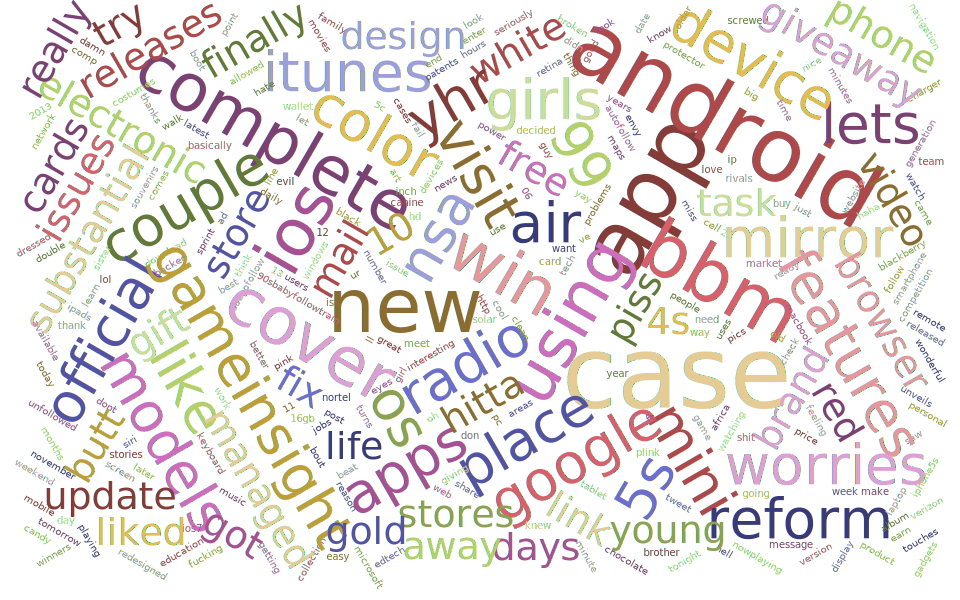
\includegraphics[scale=0.75,angle=90]{Figures/40_topics_cloud}
\end{center}
\caption{A word cloud of all tokens from all topics in our 40-topics model}
\label{fig:40-topics-cloud}
\end{figure}

\begin{longtable}{c p{16cm}} \toprule
  Topic & Topic-Words associations \\ \midrule
   0    & big, year, chocolate, mobile, gadgets, double, boot, girls like, white girls, touches \\ \midrule
   1    & app, store, know, available, does, design, stargazing, stargazing app, ft, new design \\ \midrule
   2    & gift, version, 25, liked, liked video, months, earn, watch, gift cards, knew \\ \midrule
   3    & follow, ip, place, walk, laptop, electronic, web, dont, competition, costumes \\ \midrule
   4    & using, hate, tweet, using app, reason, bout, thing, unfollowed using, case like, girl \\ \midrule
   5    & white, education, giveaway, tablet, comes, brand, brand new, way, halloween giveaway, win plink \\ \midrule
   6    & visit, place visit, visit gameinsight, ipads, place, unveils, power, rivals, stories case \\ \midrule
   7    & video, download, 16gb, black, watching, nowplaying, clean, smartphone, eyes, sprint \\ \midrule
   8    & great, giving, yay, miss, post, feeling, turns, maps, keyboard, canine evil \\ \midrule
   9    & number, tfbjp teamfairyrose, retweet tfbjp, sougofollow, teamfairyrose, autofollow, 06, cards, 90sbabyfollowtrain, interesting \\ \midrule
   10   & ios, official, 5s, like, world, game, facebook, new 5s, cool, africa \\ \midrule
   11   & new, gameinsight, try, updated, try gameinsight, achievement, new achievement, jobs, achievement 10, areas \\ \midrule
   12   & android, need, use, blackberry, devices, hd, problems, card, art, issue \\ \midrule
   13   & bbm, bbm android, official release, android official, got, want, gold, macbook, gold 5s, smart \\ \midrule
   14   & apps, lets, bbm ios, ios lets, lets apps, phone, don, best, people, meet \\ \midrule
   15   & missed, having, app android, case missed, windows, 12, daily, cell, apps android, decided \\ \midrule
   16   & perfect, android bbm, perfect features, features bbm, love, collection, pink, did, let, website \\ \midrule
   17   & samsung, google samsung, backed, entirely, nortel, patents, share, beat, uses, really entirely \\ \midrule
   18   & mini, win, chance, chance win, models red, kickstand case, mini models, targus, targus kickstand, case mini \\ \midrule
   19   & air, http, better, young, news, mirror, market, mirror world, souvenirs mirror, envy complete \\ \midrule
   20   & retina, device, red, electronic device, device using, ur, inch, 13, fix, wallet \\ \midrule
   21   & pc, life, old, releases, saywhatnow, releases air, air saywhatnow, cases, away, battery life \\ \midrule
   22   & check, music, 10, mavericks, generation, os mavericks, ready, fix issues, mail, mail update \\ \midrule
   23   & case, buy, cover, 99, end, 2013, case 4s, case cover, smart cover, cover case \\ \midrule
   24   & haha, isn, line, allowed, oh, solar, price, android phone, guy, basically \\ \midrule
   25   & app, just, radio, updated ios, users, young hitta, yhr app, yhr, radio yhr, hitta radio \\ \midrule
   26   & os, stores, playing, latest, hours, fail, piss, stores piss, issues, protector \\ \midrule
   27   & release, halloween, 5c, work, models, days, online, product, color, pics \\ \midrule
   28   & battery, lol, good, shit, thanks, tomorrow, ios7, minutes, minute, november \\ \midrule
   29   & itunes, released, think, thank, album, downloadtoyboysingle, itunes link, downloadtoyboysingle itunes, saw, sister \\ \midrule
   31   & ll, charger, didn, personal, later, nice, brother, movies, butt, butt away \\ \midrule
   32   & features, tech, make, cracked, worries, color highlighters, cracked worries, highlighters, worries color, say \\ \midrule
   33   & complete, 4s, , managed, week, display, girls, task, managed complete, complete task \\ \midrule
   34   & free, enter, win, 99 free, app 99, iphone5s, navigation, comp, fucking, network \\ \midrule
   35   & really, update, broken, damn, 11, family, seriously, point, message, took \\ \midrule
   36   & time, retweet, date, wonderful, hell, edtech, learn, screwed, winners chosen, chosen tonight \\ \midrule
   36   & today, ve, going, verizon, couple, couple days, team couple, dressed, came, online store \\ \midrule
   37   & screen, finally, look, years, getting, weekend, remote, siri, finally got, ad redesigned \\ \midrule
   38   & google, nsa, microsoft, reform, reform nsa, substantial, substantial reform, surveillance, facebook google, nsa surveillance \\ \midrule
   39   & day, easy, link, older, candy, browser, os browser, otterbox, defender, otterbox defender \\ \bottomrule
\caption{40 word-topic distributions with unigrams and bigrams}
\label{tab:40-topics}
\end{longtable}


